\documentclass[xetex,mathserif,serif]{beamer}
\usepackage{polyglossia}
\setdefaultlanguage[babelshorthands=true]{russian}
\usepackage{minted}
\usepackage{tabu}

\useoutertheme{infolines}

\usepackage{fontspec}
\setmainfont{FreeSans}
\newfontfamily{\russianfonttt}{FreeSans}

\tabulinesep=0.8mm

\title{Графический интерфейс на Java}
\author[Юрий Литвинов]{Юрий Литвинов \newline \textcolor{gray}{\small\texttt{yurii.litvinov@gmail.com}}}

\date{20.04.2017г}

\begin{document}
	
	\frame{\titlepage}
	
	\section{Введение}

	\begin{frame}
		\frametitle{Оконные библиотеки для Java}
		\begin{itemize}
			\item AWT --- очень старая, основа Swing
			\item Swing --- старая, но очень популярна
			\item SwingX --- расширение Swing
			\item JavaFX --- с Java8 стандарт де-факто
			\item Apache Pivot --- прежде всего для веб-приложений
			\item Qt Jambi --- binding-и к Qt, требует нативных библиотек
			\item SWT --- требует нативных библиотек
		\end{itemize}
	\end{frame}

	\section{JavaFX}

	\begin{frame}
		\frametitle{JavaFX}
		\begin{center}
			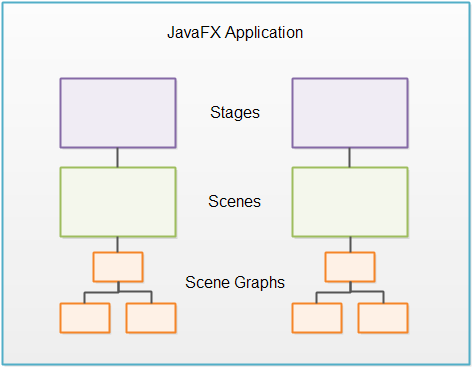
\includegraphics[width=0.6\textwidth]{javaFxOverview.png}
		\end{center}
	\end{frame}

	\begin{frame}[fragile]
		\frametitle{Минимальный пример}
		\begin{minted}{java}
import javafx.application.Application;
import javafx.stage.Stage;

public class MyFxApp extends Application {
    @Override
    public void start(Stage primaryStage) throws Exception {
        primaryStage.setTitle("My First JavaFX App");
        primaryStage.show();
    }
    
    public static void main(String[] args) {
        Application.launch(args);
    }
}
		\end{minted}
\end{frame}

	\begin{frame}[fragile]
		\frametitle{Кнопки}
		\begin{minted}{java}
public class ButtonExperiments extends Application  {
    @Override
    public void start(Stage primaryStage) throws Exception {
        Button button = new Button("Click me");

        button.setOnAction(value -> Platform.exit());

        Scene scene = new Scene(button, 200, 100);
        primaryStage.setScene(scene);
        primaryStage.show();
    }

    public static void main(String[] args) {
        Application.launch(args);
    }
}
		\end{minted}
\end{frame}

	\begin{frame}
		\frametitle{Лейауты}
			\begin{tabu} {| X[1 l m] | X[1 c m] |}
				\tabucline-
				\everyrow{\tabucline-}
				BorderPane               & 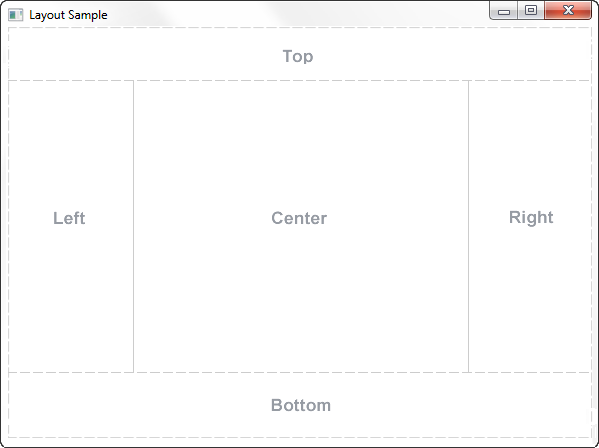
\includegraphics[height=0.2\textheight]{borderLayout.png}           \\
				HBox                     & 
\includegraphics[height=0.04\textheight]{hbox.png}                  \\
				VBox                     &                                                                     \\
				GridPane                 & 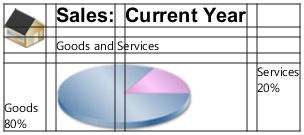
\includegraphics[height=0.1\textheight]{grid.png}                   \\
				AnchorPane               & 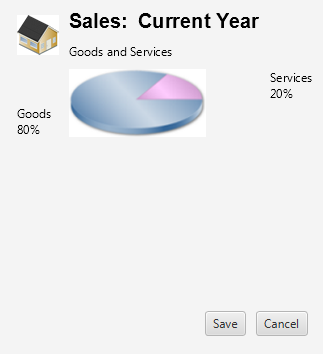
\includegraphics[height=0.2\textheight]{anchor.png}                 \\
				...                      & 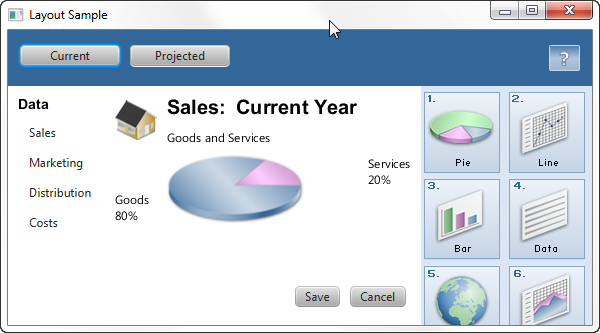
\includegraphics[height=0.1\textheight]{anchor_in_border_small.png} \\
			\end{tabu}
	\end{frame}

	\begin{frame}
		\frametitle{Элементы управления}
		\framesubtitle{Controls}
		\begin{center}
			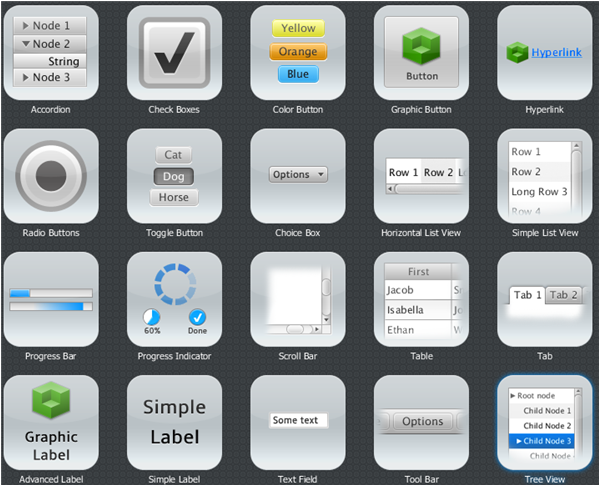
\includegraphics[width=0.6\textwidth]{javaFxControls.png}
		\end{center}
	\end{frame}

	\begin{frame}
		\frametitle{Стили}
		\framesubtitle{CSS}
		\begin{center}
			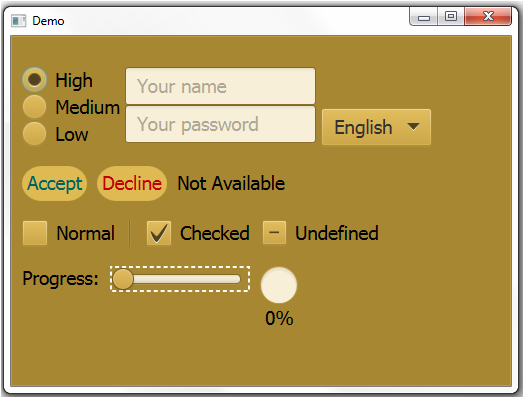
\includegraphics[width=0.6\textwidth]{styles.png}
		\end{center}
	\end{frame}

	\begin{frame}[fragile]
		\frametitle{Пример, установка стиля}
		Java:
		\begin{minted}{java}
Scene scene = new Scene(new Group(), 500, 400);
scene.getStylesheets().add("path/stylesheet.css");
		\end{minted}
		\vspace{1cm}
		CSS (path/stylesheet.css):
		\begin{minted}{css}
.custom-button {
    -fx-font: 16px "Serif";
    -fx-padding: 10;
    -fx-background-color: #CCFF99;
}
		\end{minted}
\end{frame}

	\begin{frame}[fragile]
		\frametitle{FXML}
		\begin{minted}{xml}
<?xml version="1.0" encoding="UTF-8"?>
<?import javafx.scene.control.*?>
<?import javafx.scene.layout.*?>
<?import javafx.scene.text.*?>
<GridPane alignment="center" hgap="10" vgap="10">
    <Text id="hello-word-text" text="Hello, world!"
            GridPane.columnIndex="0"
            GridPane.rowIndex="0" GridPane.halignment="CENTER"/>
    <Button text="Ok" GridPane.columnIndex="0"
            GridPane.rowIndex="1" GridPane.halignment="CENTER"/>
</GridPane>
		\end{minted}
\end{frame}

	\begin{frame}[fragile]
		\frametitle{FXML, в коде}
		\begin{minted}{java}
public class FXMLExample extends Application {
    @Override
    public void start(Stage stage) throws Exception {
        Parent root = FXMLLoader.load(
            new File("fxmlExample.fxml").toURI().toURL());

        stage.setTitle("FXML Welcome");
        stage.setScene(new Scene(root, 300, 275));
        stage.show();
    }

    public static void main(String[] args) {
        Application.launch(FXMLExample.class, args);
    }
}
		\end{minted}
\end{frame}

	\section{Задания}

	\begin{frame}
		\frametitle{Домашка, GUI к FTP}
		Сделать GUI для FTP-клиента, позволяющий ходить по дереву файлов с сервера и скачивать файлы
		\begin{itemize}
			\item Можно пользоваться JavaFX или Swing
			\item Дедлайн: \textbf{03.05.2017 23:59}
		\end{itemize}
	\end{frame}

	\begin{frame}
		\frametitle{Задание на остаток пары, крестики-нолики}
		Разработать приложение, позволяющие пользователю играть с самим собой в крестики-нолики. 
		\begin{itemize}
			\item На экранной форме должно быть 9 кнопок, расположенных в три столбца и три строки
			\item При первоначальном нажатии на любую из кнопок, на ней появляется знак <<Х>> 
			\item При дальнейшем нажатии на другую кнопку, на ней появляется знак <<O>>
			\item Повторное нажатие на кнопку не должно менять ее знака
		\end{itemize}
	\end{frame}

	\section{Заключение}

	\begin{frame}
		\frametitle{Полезные ссылки}
		\begin{itemize}
			\item \url{http://tutorials.jenkov.com/javafx/index.html}
			\item \url{http://docs.oracle.com/javase/8/javase-clienttechnologies.htm}
			\item \url{http://docs.oracle.com/javafx/2/get_started/fxml_tutorial.htm}
		\end{itemize}
	\end{frame}

\end{document}
